\style{mb} %pour microbit


%   Titre de la sous sections
\section{Normal ou truqué? avec \mb}
%   logo mb dans la table des matières
%\logo{mb}

%
%   style de la page
%   commenter avec % le style non utilisé
%\pagestyle{st} %pour ST

\subsection{Description}

\subsubsection{Objectif}


%   bloc de formule
%   sans titre et fond bleu cyan
\begin{formule}
Cette activité propose à l'élève de travailler sur la \emph{fluctuation d'échantillonnage}.

Sans accéder au code, seulement \emph{en manipulant} la carte \mb, l'élève doit déterminer si le jeu téléversé est un jeu \emph{normal} ou \emph{truqué}\ldots
\end{formule}


\subsubsection{Intérêt}

L'intérêt de cette activité est de pouvoir, en toute liberté, créer des situations équiprobables ou non. Même s'il est possible d'utiliser de vrais dès truqués, l'utilisation d'une carte \mb permet un éventail très larges de situations.

Ici le choix a été fait de procéder à un tirage aléatoire (ou non ;) ) d'un nombre entre 0 et 9 (inclus).


\subsubsection{Matériel}
\begin{itemize}
%   matériel pour micro:bit
    \item 1 $\times$ \matosMb \emph{(facultatif car le simulateur peut suffire)}
%   site pour micro:bit
    \item 1 $\times$ accès internet : IDE programmation par bloc \url{http://makecode.microbit.org/}
\end{itemize}



\subsubsection{Progression}

L'activité se déroule en 2 temps :
\begin{description}
    \item[Analyse du programme] Dans cette partie, l'élève doit étudier les deux programmes possibles (truqué ou non) puis répondre à une série de questions de probabilités
    \item[Expérience aléatoire] Ensuite l'élève manipule la carte \mb et effectue un certain nombre d'expériences aléatoires. Dans cette partie l'analyse des échantillons et la création d'une représentation graphique permettra de conclure sur le type de programme téléversé.
\end{description}

%
% activité de niveau 
%

%   saut de page
\newpage

%   titre de la sous section
\subsection{Activité}

\subsubsection{Activité élève}

% commande perso \CARTOUCHE
%   5 paramètres : 
%       * durée
%       * public
%       * travail en maths
%       * travail en sciences
%       * travail en algo
\cartouche
{2 h}         %durée
{2de ; term}           %public
{fluctuation d'échantillage}        %maths
{}     %sciences
{}       %algo


%   petite image de logo qui va
%   se mettre dans le bloc élève
\begin{wrapfigure}[4]{r}{2cm}\rule{0cm}{2pt}
    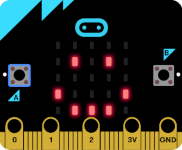
\includegraphics[width=\linewidth]{res/mb-truque-mini.png}
\end{wrapfigure}

%   bloc élève
%   fond orange
\begin{eleve}    
    \texttt{\textsc{Normal ou \emph{truqué} ?}}
    
    Sur votre carte est téléversé un des deux programmes de jeu suivant. Quand le joueur gagne, il a un smiley sourire, sinon il a  une croix. 
    
    
    
%   ajout d'une image
\begin{minipage}[t]{0.5\linewidth}
    \begin{center}
        \vspace{0cm}
        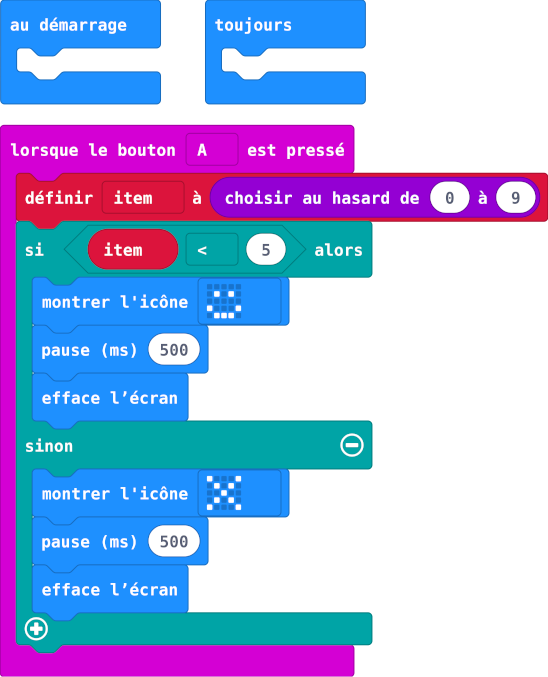
\includegraphics[width=0.7\linewidth]{res/mb-normal.png}\\
        Jeu \emph{normal}
    \end{center}
\end{minipage}
\hfill
\begin{minipage}[t]{0.5\linewidth}
    \begin{center}
        \vspace{0cm}
        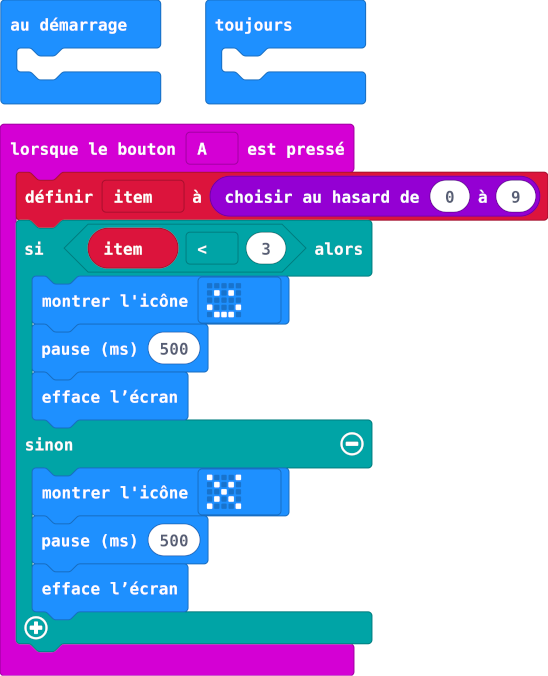
\includegraphics[width=0.7\linewidth]{res/mb-truque.png}\\
        Jeu \emph{truqué}
    \end{center}
\end{minipage}
    
    \textbf{Analyse du programme}
    
    \begin{enumerate}
        \item   Si on choisit un nombre entier au hasard entre 0 et 9, combien y-a-t-il d’issues possibles ?
        \item Si pour gagner il faut obtenir un nombre entre 0 et 4, combien y-a-t-il d’issues favorables ?  
        \item Calculer la probabilité de gagner avec la version normale du programme. Donner le résultat sous forme de fraction, de nombre décimal et de pourcentage.
        \item Avec le même raisonnement, calculer la probabilité de gagner avec la version truquée du programme. Donner le résultat sous forme de fraction, de nombre décimal et de pourcentage.
    \end{enumerate}
    
    \newpage
    \textbf{Analyse du programme}
    
    \begin{enumerate}
        \setcounter{enumi}{4}
        \item \emph{Jouer des parties} par séquence de 25 parties et noter G pour gagner et P pour perdu, dans votre cahier.
        \item En utilisant vos résultats, compléter le tableau ci-dessous. \emph{Attention !} Bien prendre son temps pour compter.\\
        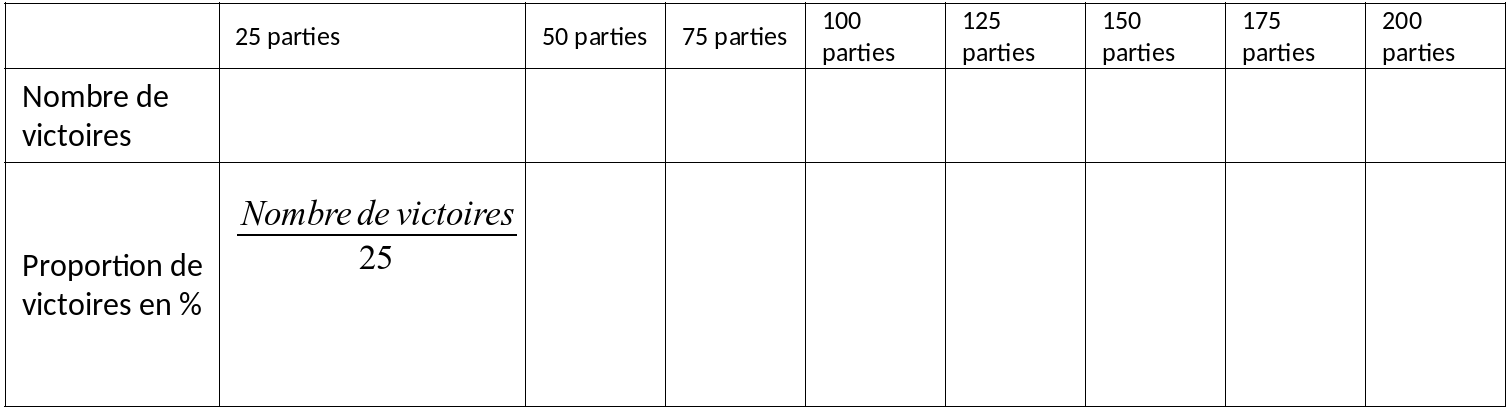
\includegraphics[width=\linewidth]{res/mb-truque-activite2.png}
        \item Compléter le graphique correspondant à la dernière ligne du tableau : placer un point par colonne, relier les points par des segments et légender les axes.\\
        Donner un \emph{titre} au graphique.\\
          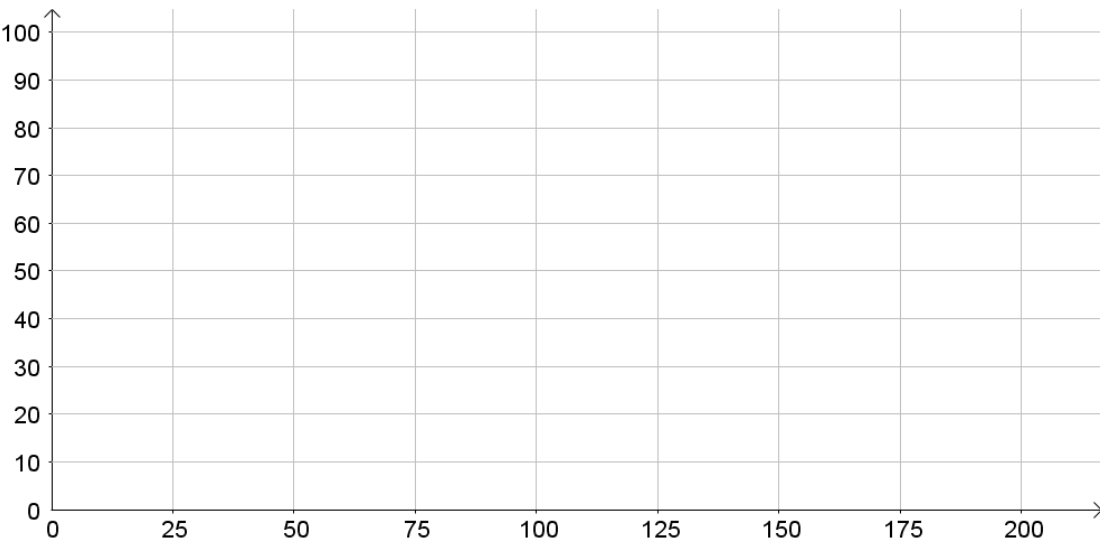
\includegraphics[width=\linewidth]{res/mb-truque-activite3.png}
        \item Analyser le graphique et conclure sur le programme qui est téléchargé dans votre carte.\\
        Argumenter avec une ou plusieurs phrases.
    \end{enumerate}
    
\end{eleve}



\subsubsection{Notes pour l'enseignant}

\begin{remarque}
    Le code \emph{interactif} est accessible en ligne : 
    \begin{description}
        \item[Jeu normal] \url{https://makecode.microbit.org/_0E1iAAee46YC}
        \item[Jeu truqué] \url{https://makecode.microbit.org/_4zFAsTUuEgYV}
    \end{description}
\end{remarque}